\documentclass{beamer}
\mode<presentation>
\usepackage{amsmath}
\usepackage{amssymb}
%\usepackage{advdate}
\usepackage{adjustbox}
\usepackage{subcaption}
\usepackage{enumitem}
\usepackage{multicol}
\usepackage{mathtools}
\usepackage{listings}
\usepackage{url}
\def\UrlBreaks{\do\/\do-}
\usetheme{Boadilla}
\usecolortheme{lily}
\setbeamertemplate{footline}
{
  \leavevmode%
  \hbox{%
  \begin{beamercolorbox}[wd=\paperwidth,ht=2.25ex,dp=1ex,right]{author in head/foot}%
    \insertframenumber{} / \inserttotalframenumber\hspace*{2ex} 
  \end{beamercolorbox}}%
  \vskip0pt%
}
\setbeamertemplate{navigation symbols}{}

\providecommand{\nCr}[2]{\,^{#1}C_{#2}} % nCr
\providecommand{\nPr}[2]{\,^{#1}P_{#2}} % nPr
\providecommand{\mbf}{\mathbf}
\providecommand{\pr}[1]{\ensuremath{\Pr\left(#1\right)}}
\providecommand{\qfunc}[1]{\ensuremath{Q\left(#1\right)}}
\providecommand{\sbrak}[1]{\ensuremath{{}\left[#1\right]}}
\providecommand{\lsbrak}[1]{\ensuremath{{}\left[#1\right.}}
\providecommand{\rsbrak}[1]{\ensuremath{{}\left.#1\right]}}
\providecommand{\brak}[1]{\ensuremath{\left(#1\right)}}
\providecommand{\lbrak}[1]{\ensuremath{\left(#1\right.}}
\providecommand{\rbrak}[1]{\ensuremath{\left.#1\right)}}
\providecommand{\cbrak}[1]{\ensuremath{\left\{#1\right\}}}
\providecommand{\lcbrak}[1]{\ensuremath{\left\{#1\right.}}
\providecommand{\rcbrak}[1]{\ensuremath{\left.#1\right\}}}
\theoremstyle{remark}
\newtheorem{rem}{Remark}
\newcommand{\sgn}{\mathop{\mathrm{sgn}}}
\providecommand{\abs}[1]{\left\vert#1\right\vert}
\providecommand{\res}[1]{\Res\displaylimits_{#1}} 
\providecommand{\norm}[1]{\lVert#1\rVert}
\providecommand{\mtx}[1]{\mathbf{#1}}
\providecommand{\mean}[1]{E\left[ #1 \right]}
\providecommand{\fourier}{\overset{\mathcal{F}}{ \rightleftharpoons}}
%\providecommand{\hilbert}{\overset{\mathcal{H}}{ \rightleftharpoons}}
\providecommand{\system}{\overset{\mathcal{H}}{ \longleftrightarrow}}
	%\newcommand{\solution}[2]{\textbf{Solution:}{#1}}
%\newcommand{\solution}{\noindent \textbf{Solution: }}
\providecommand{\dec}[2]{\ensuremath{\overset{#1}{\underset{#2}{\gtrless}}}}
\newcommand{\myvec}[1]{\ensuremath{\begin{pmatrix}#1\end{pmatrix}}}
\let\vec\mathbf

\lstset{
%language=C,
frame=single, 
breaklines=true,
columns=fullflexible
}

\numberwithin{equation}{section}

\title{2.5.20}
\author{Rushil Shanmukha Srinivas \\EE25BTECH11057 \\ Electrical Enggineering ,\\IIT Hyderabad.}

\date{\today} 
\begin{document} 

\begin{frame}
\titlepage
\end{frame}

\section*{Outline}
\begin{frame}
\tableofcontents
\end{frame}
\section{Problem}
\begin{frame}
\frametitle{Problem Statement}

Let $\vec a,\vec b,\vec c$ be three vectors with $\lVert \vec a\rVert=1,\ \lVert\vec b\rVert=2,\ \lVert\vec c\rVert=3$. 
If the projection of $\vec b$ on $\vec a$ equals the projection of $\vec c$ on $\vec a$, and $\vec b\perp\vec c$, find

$\bigl\lVert 3\vec a-2\vec b+2\vec c\bigr\rVert.$

\end{frame}
\section{Solution}
\subsection{Dot Product of vectors}
\begin{frame}
\frametitle{Dot Product of vectors}
%\framesubtitle{Literature}
Let us denote the scalar products
\begin{align}
x=\vec a\cdot\vec b,\qquad y=\vec a\cdot\vec c,\qquad z=\vec b\cdot\vec c .
\end{align}
Given: projection of $\vec b$ on $\vec a$ equals projection of $\vec c$ on $\vec a$.
Since $\lVert\vec a\rVert=1$, this implies
\begin{align}
\vec a\cdot\vec b=\vec a\cdot\vec c \quad\Rightarrow\quad x=y.
\end{align}
Also $\vec b\perp\vec c\Rightarrow z=0$. Using the magnitudes,
\begin{align}
\vec a\cdot\vec a=1,\quad \vec b\cdot\vec b=4,\quad \vec c\cdot\vec c=9.
\end{align}

\end{frame}
\subsection{Gram Matrix}
\begin{frame}
\frametitle{Gram Matrix}
Form the Gram (inner-product) matrix of $(\vec a,\vec b,\vec c)$:
\begin{align}
G=\myvec
{\vec a\cdot\vec a & \vec a\cdot\vec b & \vec a\cdot\vec c\\
\vec b\cdot\vec a & \vec b\cdot\vec b & \vec b\cdot\vec c\\
\vec c\cdot\vec a & \vec c\cdot\vec b & \vec c\cdot\vec c}
=
\myvec
{1 & x & x\\
x & 4 & 0\\
x & 0 & 9}
,
\end{align}
where we used $x=y$ and $z=0$.

Now denote the coefficient vector of $3\vec a-2\vec b+2\vec c$ relative to $(\vec a,\vec b,\vec c)$ by
\begin{align}
\mathbf{u}=\myvec{3\\-2\\2}.
\end{align}
Then the squared norm is the quadratic form
\begin{align}
\bigl\lVert 3\vec a-2\vec b+2\vec c\bigr\rVert^2
= \mathbf{u}^\top G\,\mathbf{u}.
\end{align}
\end{frame}

\begin{frame}
\begin{align}
\mathbf{u}^\top G\, \mathbf{u}
=\myvec
{3 & -2 & 2}
\myvec
{1 & x & x\\
x & 4 & 0\\
x & 0 & 9}
\myvec 
{3\\-2\\2 }
=9 -6x +16 +6x +36 =61
\end{align}

Therefore
\begin{align}
\bigl\lVert 3\vec a-2\vec b+2\vec c\bigr\rVert^2 = 61
\quad\Longrightarrow\quad
\boxed{\bigl\lVert 3\vec a-2\vec b+2\vec c\bigr\rVert=\sqrt{61}}.
\end{align}
\end{frame}

\subsection{Plots}
\begin{frame}
\frametitle{Plots}
\begin{figure}
\centering
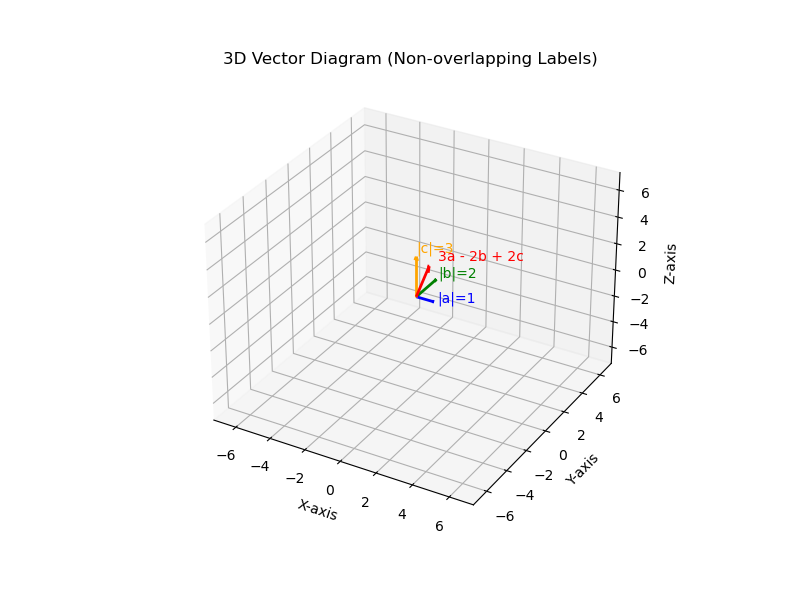
\includegraphics[width=0.9\columnwidth]{figs/fig3.png}
\caption{fig : Representation of vectors}
\label{Fig3}
\end{figure}
\end{frame}
\section{C Code}
\begin{frame}[fragile]
\frametitle{C Code }
\begin{lstlisting}[language=C]

#include <stdio.h>
#include <math.h>

// Function to compute magnitude of (3a - 2b + 2c)
double compute_magnitude() {
    // Given norms
    double norm_a = 1.0;
    double norm_b = 2.0;
    double norm_c = 3.0;


    double result_squared =
        9 * (norm_a * norm_a) +       // 9|a|^2
        4 * (norm_b * norm_b) +       // 4|b|^2
        \end{lstlisting}
        \end{frame}
        \begin{frame}[fragile]
        \begin{lstlisting}
        4 * (norm_c * norm_c) +       // 4|c|^2
        -12 * (0) + 12 * (0) + -8 * (0);

    // Simplified: 9*1 + 4*4 + 4*9 = 61
    return sqrt(result_squared);
}

int main() {
    double magnitude = compute_magnitude();
    printf("The magnitude of (3a - 2b + 2c) is: %.5f\n", magnitude);
    return 0;
}
    
\end{lstlisting}
\end{frame}

\section{Python Code}
\begin{frame}[fragile]
\frametitle{Python : call\_c.py}
\begin{lstlisting}
import ctypes
import os
import math
# Load the shared library (ensure libvector.so is in the same directory)
lib_path = os.path.abspath("./libvector.so")
lib = ctypes.CDLL(lib_path)
# Tell Python the return type of the C function
lib.compute_magnitude.restype = ctypes.c_double
# Call the function from the shared object
result = lib.compute_magnitude()
# Print result
print("The magnitude of (3a - 2b + 2c) is:", result)

# (Optional) Verify using Python math
print("Verification using Python math.sqrt(61):", math.sqrt(61))

\end{lstlisting}
\end{frame}

\begin{frame}[fragile]
\frametitle{Python Code for Plotting}
\begin{lstlisting}[language=Python]
import numpy as np
import matplotlib.pyplot as plt
from mpl_toolkits.mplot3d import Axes3D

# Step 1: Define vectors
a = np.array([1, 0, 0])   # |a| = 1
b = np.array([0, 2, 0])   # |b| = 2
c = np.array([0, 0, 3])   # |c| = 3

# Required vector
v = 3*a - 2*b + 2*c

# Step 2: Setup 3D figure
fig = plt.figure(figsize=(8,6))
ax = fig.add_subplot(111, projection='3d')
\end{lstlisting}
\end{frame}
\begin{frame}[fragile]
\begin{lstlisting}
# Helper function to draw vectors with shifted labels
def draw_vector(ax, origin, vec, color, label, shift):
    ax.quiver(
        origin[0], origin[1], origin[2],
        vec[0], vec[1], vec[2],
        color=color, arrow_length_ratio=0.1, linewidth=2
    )
    ax.text(
        vec[0] + shift[0],
        vec[1] + shift[1],
        vec[2] + shift[2],
        label,
        fontsize=10, color=color
    )

# Step 3: Plot vectors with shifted labels
draw_vector(ax, [0,0,0], a, "blue",   "|a|=1",    shift=[0.2,0,0])
draw_vector(ax, [0,0,0], b, "green",  "|b|=2",    shift=[0,0.2,0])
\end{lstlisting}
\end{frame}
\begin{frame}[fragile]
\begin{lstlisting}
draw_vector(ax, [0,0,0], c, "orange", "|c|=3",    shift=[0,0,0.3])
draw_vector(ax, [0,0,0], v, "red",    "3a - 2b + 2c", shift=[0.3,0.3,0.3])

# Step 4: Axis settings
max_range = np.max(np.abs([a, b, c, v])) + 1
ax.set_xlim([-max_range, max_range])
ax.set_ylim([-max_range, max_range])
ax.set_zlim([-max_range, max_range])

ax.set_xlabel("X-axis")
ax.set_ylabel("Y-axis")
ax.set_zlabel("Z-axis")
ax.set_title("3D Vector Diagram (Non-overlapping Labels)")

plt.show()
\end{lstlisting}
\end{frame}

\end{document}